\chapter{Realizability Problems for Weighted Trees}\label{chp:disk}

We begin this chapter with the preliminary concepts to solving Problems \ref{problem:UnorderedContactGraph} and \ref{problem:OrderedContactGraph}, and then prove related Theorem \ref{thm:disk}.  
Recall the Unordered and Ordered Realizability Problem for a contact graph  and corresponding theorem which state:

\begin{itemize}
\item[\textbf{Problem \ref{problem:UnorderedContactGraph}}] Given a planar graph with positive weighted vertices, is it a contact graph of some disk arrangement where the radii equal the vertex weights?
\item[\textbf{Problem \ref{problem:OrderedContactGraph}}] Given a planar graph with positive weighted vertices and a combinatorial embedding, is it a contact graph of some disk arrangement where the radii equal the vertex weights and the counter-clockwise order of neighbors of each disk is specified by the combinatorial embedding?
\item[\textbf{Theorem \ref{thm:disk}}] It is NP-Hard to decide whether a given tree with positive vertex weights
is the contact graph of a disk arrangements with specified radii.
\end{itemize}

In this chapter, we will show the following lemma:
  
The preliminary concepts for Disk Arrangements are the Unit Disk Touching Graph Recongnition Problem, the Perturbed Root with Unit Disk Leaves Touching Graph Recongnition Problem, and Hausdorff distance.  
All together the preliminary concepts will allow us to approximate the geometry of polygons and allow us to use the results of the polygonal linkages in Chapter \ref{chapter:polygonalLinkage}.

%\chapter{Disk Arrangement}
\section{Properties for Weighted Trees and Polygonal Linkages}
In order to perform our analysis for weighted trees and polygonal linkages, we'll want to use a suitable metric.  The usual Euclidian distance will not suffice for this analysis and so we turn to the Hausdorff distance.
\paragraph{Hausdorff Distance}  Let $A$ and $B$ be sets in the plane. The \textit{directed Hausdorff distance} is 
\begin{equation}\label{eqn:ContactGraphV3-1}
d\lr{A,B} = \sup_{a \in A} \inf_{b \in B} \left\vert\left\vert a-b \right\vert \right\vert
\end{equation}
$h\lr{A,B}$ finds the furthest point $a in A$ from any point in $B$.  \textit{Hausdorff distance} is
\begin{equation}\label{eqn:ContactGraphV3-2}
D\lr{A,B} = \max \left\lbrace d\lr{A,B}, d\lr{B,A} \right\rbrace
\end{equation}
\begin{figure}[!htbp]
\begin{center}
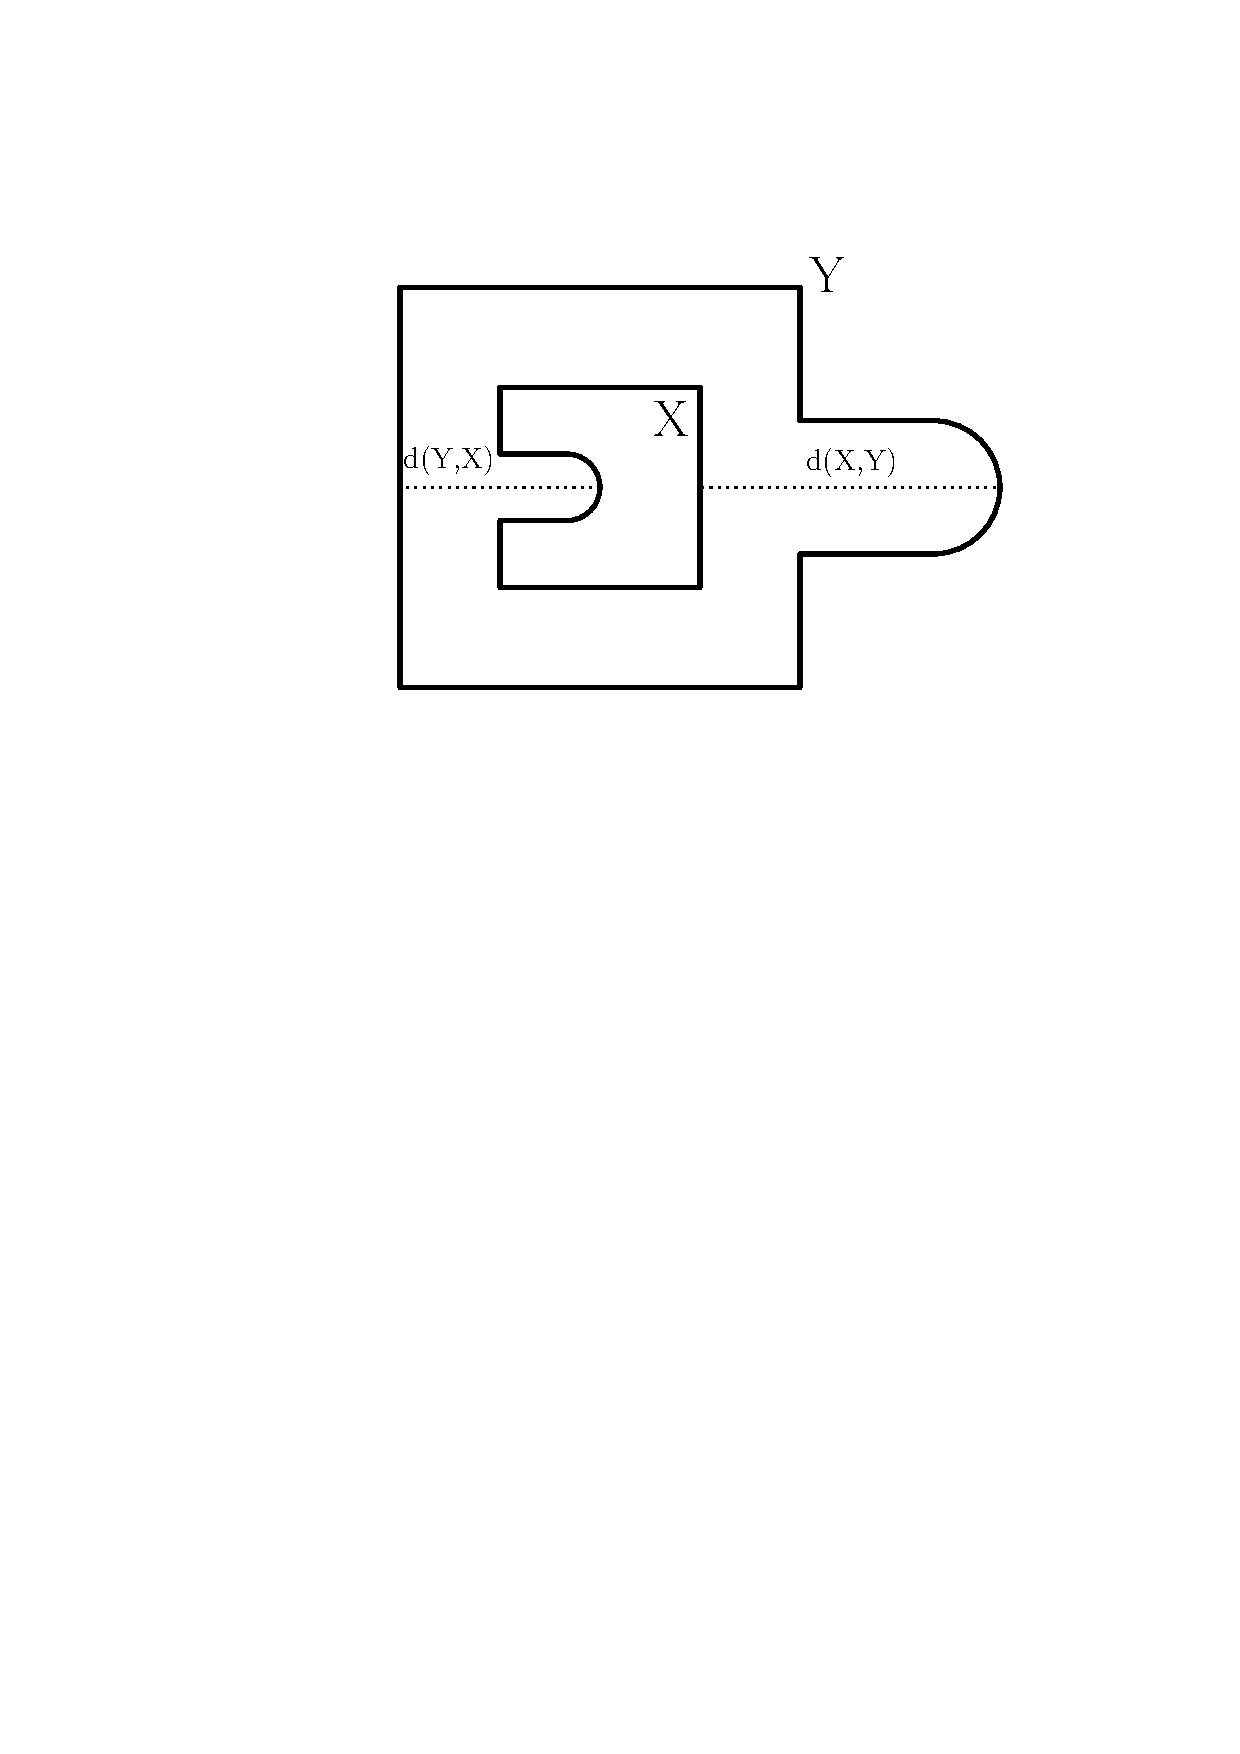
\includegraphics[scale=.5]{graphics/HausdorffDistanceExample1.pdf}
\caption{An illustrative example of $d(X,Y)$ and $d(Y,X)$ where $X$ is the inner curve, and $Y$ is the outer curve.}\label{fig:HausdorffDistanceExample1.pdf}
\end{center}
\end{figure}
\paragraph{$\epsilon$-approximation}
% Modeling the logic engine with polygonal linkages requires reflected copies of the
% rectangles. For an oriented realization, we use a different technique in Section 3. The
% above proof can be adapted to the realization of contact trees of disks by approximating
% rectangles with disk arrangements. In this context, we say that a weighted graph G is a
% ε-approximation of a polygon P if G is realizable as a contact graph of disks of given
% radii, and in every such realization, the Hausdorff distance between the union of disks
% and a congruent copy of P is at most ε. A weighted graph G is a stable ε-approximation
% if, in addition, for every two such realizations of G, the distance between the centers of
% the corresponding disks is at most ε after a suitable rigid transformation.
The weighted graph, $G$, is an \textit{$\epsilon$-approximation} of a polygon $P$ if the Hausdorff distance between every realization such realization of $G$ as a contact graph of disks and a congruent copy of $P$ is at most epsilon.  A weighted graph $G$ is said to be a \textit{$\BigOh{f(x)}$-approximation} of a polygon P if there is a positive constant $M$ such that for all sufficiently large values of $x$ the Hausdorff distance between every realization such realization of $G$ as a contact graph of disks and a congruent copy of $P$ is at $M \cdot \vert f(x)\vert$. A weighted graph $G$ is said to be a \textit{stable} if it has the property that for every two such realizations of $G$, the distance between the centers of the corresponding disks is at most $\epsilon$ after a suitable rigid transformation.  
\section{Unit Disk Touching Graph Recongnition Problem (UDTGRP)}

% Lemma 3. For every instance $\Phi$ of P3SAT, the corresponding modified auxiliary construction
% has the following properties: (1) it has polynomial size; (2) the hinge graph of the modified auxilary con-
% struction is a tree; (3) it admits a realization such that the obstacle polygons remain fixed if and only if $\Phi$ is
% satisfiable.

The UDTGRP is to determine when given an instance of a weighted graph (V,E) where each vertex has unit weight can be realized as a disk touching graph (a disk arrangement).  

In this section we describe a particular family of unit weight graphs and corresponding disk arrangements called \textit{snowflakes}.
Note that we regard snowflakes with unit weight as a weight of $\frac{1}{2}$.
For $i \in \bbN$, the construction of the snowflake tree, $S_i$, is as follows:
\begin{itemize}
\item Let $v_0$ be a vertex that has six paths attached to it: $p_1$, $p_2$, $\dots$, $p_6$.  Each path has $i$ vertices.
\item For every other path $p_1$, $p_3$, and $p_5$: 
	\begin{itemize}
		\item 	Each vertex on that path has two paths attached, one path on each side of $p_k$.
		\item	The number of vertices that lie on a path attached to the $j^\text{th}$ vertex of $p_k$ is $i-j$.
	\end{itemize}
\end{itemize}

\begin{figure}[!htbp]
\begin{center}
\includegraphics{graphics/snowflakeOutline5LayerSmall.pdf}
\caption{The same contact graph as in figure \ref{fig:hexagonOutline5LayerSmall.pdf} overlayed with the a perfectly weighted snowflake tree.}\label{fig:snowflakeOutline5LayerSmall.pdf}
\end{center}
\end{figure}

A \textit{perfectly weighted snowflake tree} is a snowflake tree with all vertices having weight $\frac{1}{2}$.  
A \textit{perturbed snowflake tree} is a snowflake tree with all vertices having weight of 1 with the exception of $v_0$;  in a perturbed snowflake tree, $v_0$ will have a weight of $\frac{1}{2} + \gamma$.  
For our analysis, all realizations of any snowflake, perfect or perturbed, shall have $v_0$ fixed at origin.  
% This is said to be the canonical position under Hausdorff distance of the snowflake tree.   

\paragraph{Perfectly Weighted Snowflake Tree.}

Consider the graph of the triangular lattice with unit distant edges:
\begin{eqnarray*}
V &=& \left\lbrace a\cdot (1,0) + b \cdot \left(\frac{1}{2},\frac{\sqrt{3}}{2}\right) : a,b \in \bbZ \right\rbrace\\
E &=& \left\lbrace \left\lbrace u,v \right\rbrace : \vert\vert u-v \vert\vert = 1 \text{ and } u,v \in V\right\rbrace
\end{eqnarray*}
The following graph, $G=(V,E)$ is said to be the \textit{unit distance graph} of the triangular lattice.  
We can show that no two distinct edges of this graph are non-crossing.  
First suppose that there were two distinct edges that crossed, $\left\lbrace u_1,v_1 \right\rbrace $ and $\left\lbrace u_2,v_2 \right\rbrace$.  
With respect to $u_1$, there are 6 possible edges corresponding to it, with each edge $\frac{\pi}{3}$ radians away from the next.  
Neither edge crosses another; and so we have a contradiction that there are no edge crossings with $\left\lbrace u_1,v_1 \right\rbrace $.  


The perfectly weighted snowflake tree that is a subgraph over the \textit{unit distance graph}, $G=(V,E)$, of the triangular lattice.  
To show this, for any $S_i$, fix $v_0 = 0 \cdot \cdot (1,0) + 0 \cdot \left(\frac{1}{2},\frac{\sqrt{3}}{2}\right)=\lr{0,0} \in V$ at origin.  
Next consider the six paths attached from origin.  
Fix each consecutive path $\frac{\pi}{3}$ radians away from the next such that the following points like on the corresponding paths: $\lr{1,0} \in p_1, \lr{\frac{1}{2} ,\frac{\sqrt{2}}{3}} \in p_2,\lr{-\frac{1}{2}\p_4,\frac{\sqrt{3}}{2}} \in p_3, \lr{-1,0} \in p4, \lr{-\frac{1}{2},-\frac{\sqrt{3}}{2}}\in p_5,\lr{\frac{1}{2},-\frac{\sqrt{3}}{2}}\in p_6$.  
For $S_i$, there are $i$ vertices on each path.  

We define the six paths from origin as follows:
\begin{eqnarray*}
p_1 &=& \set{a\cdot\lr{1,0} = \vec{v}}{a \in \bbR^+}\\
p_2 &=& \set{a\cdot\lr{\frac{1}{2},\frac{\sqrt{3}}{2}} = \vec{v}}{a \in \bbR^+}\\
p_3 &=& \set{-a\cdot \lr{1,0} + a \cdot \lr{\frac{1}{2},\frac{\sqrt{3}}{2}} = a\lr{-\frac{1}{2},\frac{\sqrt{3}}{2}} = \vec{v}}{a \in \bbR^+}\\
p_4 &=& \set{a \cdot \lr{-1,0} = \vec{v}}{a \in \bbR^+}\\
p_5 &=& \set{a \cdot \lr{-\frac{1}{2},-\frac{\sqrt{3}}{2}}  = \vec{v}}{a \in \bbR^+}\\
p_6 &=& \set{ a\cdot \lr{1,0} - a \cdot \lr{\frac{1}{2},\frac{\sqrt{3}}{2}}= a \cdot \lr{\frac{1}{2}, -\frac{\sqrt{3}}{2}}}{a \in \bbR^+} 
\end{eqnarray*}
For $S_i$ there exists $i$ vertices on each path.  
We shall denote the $i^\text{th}$ vertex on the $j^\text{th}$ path as $v_{j,i}$.  
For each path defined above, the paths are defined as a set of vectors, $\vec{v} = a \cdot \vec{p}$  for some $a \in \bbR^+$ and $\vec{p} \in \bbR^2$.  
By setting $a = 1,2,\dots, i$, we obtain points that are contained in $V$.  
For $j = 1,3,5$ and $l = 1,..., i$, there exists two paths attached to each vertex $v_{j,l}$.  
We borrow the term \textit{petiole} from botany to describe the two paths attached to $v_{j,l}$.
In botany, the stalk that attaches to a stem of a plant is called a petiole; petioles usually have leaves attached to their ends.
For $S_i$, each petiole attached to the $k^\text{th}$ vertex of $p_j$, there are $i-k$ vertices.  
We will need to show that each of the $i-k$ vertices on each corresponding path are also in $V$.

The triangular lattice is symmetric under rotation about $v_0$ by $\frac{\pi}{3}$ radians.  
For each vertex $v_{1,l}$ for $l=1,2,..., i-k$, we place two petioles from it; the first petiole $\frac{\pi}{3}$ above $p_1$ at $v_{1,l}$ and $\frac{-\pi}{3}$ below $p_1$ at $v_{1,l}$ and call these petioles $p_{1,l}^+$ and $p_{1,l}^-$ respectively.  
With respect to $v_{1,l}$, one unit along $p_{1,l}^+$ is a point on the triangular lattice and similarly so on $p_{1,l}^-$.  
Continuing the walk along these paths, unit distance-by-unit distance, we obtain the next point corresponding point on the the triangular lattice up to $i-k$ distance away from $v_{1,l}$.  
This shows that each of the $i-k$ vertices on $p_{1,l}^-$ and $p_{1,l}^+$ are in $V$.  
By rotating all of the paths along $p_1$ by $\frac{2\pi}{3}$ and $\frac{4\pi}{3}$, we obtain the the paths along $p_3$ and $p_5$ respectively, completing the construction.

In Figure \ref{fig:hexagonOutline5LayerSmall.pdf}, we have a set of unit radius disks arranged in a manner that outlines regular, concentric hexagons.
\begin{figure}[!htbp]
\begin{center}
\includegraphics{graphics/hexagonOutline5LayerSmall.pdf}
\caption{A contact graph that resembles the shape of concentric hexagons.}\label{fig:hexagonOutline5LayerSmall.pdf}
\end{center}
\end{figure}
\section{Perturbed Root with Unit Disk Leaves Touching Graph Recongnition Problem (PRUDTGRP)}

The PRUDTGRP is to determine when given an instance of a weighted tree (V,E) where each vertex has unit weight with the exception of the root vertex having weight $\frac{1}{2}+\gamma$ where $\gamma>0$ can be realized as a disk touching graph (a disk arrangement).  

The perturbed snowflake follows the construction of the perfect snowflake with the exception of $v_0$ having weight $\frac{1}{2} + \gamma$ where $\gamma > 0$.
A perturbed snowflake realization has some distinct qualities from perfect snowflake realizations.  
The angular relationships between adjacent vertices may vary; the distance between adjacent and neighboring vertices may vary as well.


In general, the perturbation $\gamma$ can modify the realization of a perfect snowflake $S_i$ in the following ways:
\begin{enumerate}
\item \textbf{Modification of $S_1$.} 

Given a instance of a perturbed snowflake with $v_0$ having weight $\frac{1}{2} + \gamma$ where $\gamma > 0$, vertices neighboring $v_0$ each have a range of placement on the plane when realizaed as a disk arrangement. 
Figure \ref{fig:modifiedContactGraph} shows a realization of $S_1$ and illustrates one such example of possible gaps, $\epsilon (\gamma)$, that could be created between adjacent disks of $S_1$ in a perfect snowflake.  

\begin{minipage}{\linewidth}
\begin{center}
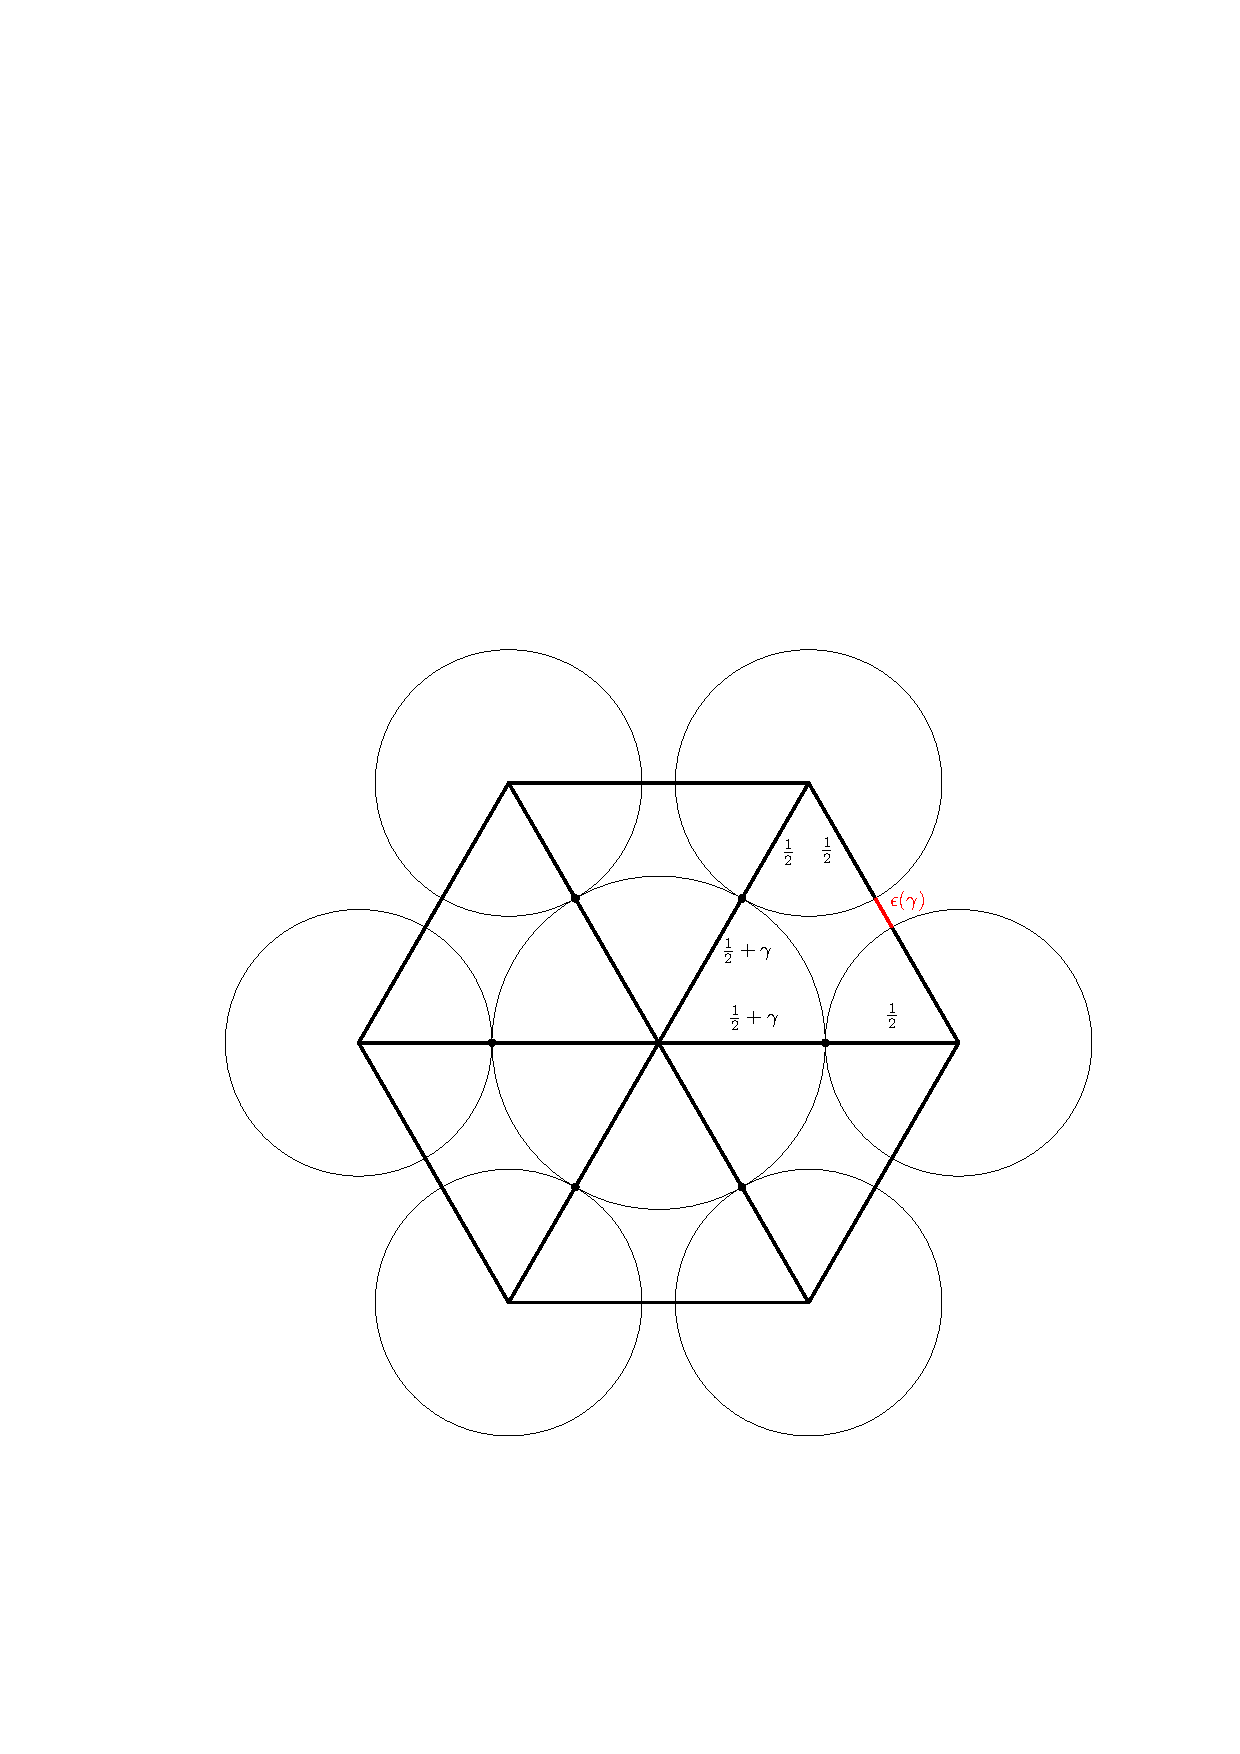
\includegraphics[width=.33\columnwidth]{graphics/modifiedContactGraph.pdf}
\captionof{figure}{A canonical disk arrangement from a perturbed snowflake with 6 unit disks around a central disk with radius $\frac{1}{2} + \gamma$.}\label{fig:modifiedContactGraph.pdf}
\end{center}
\end{minipage}

Note that (1) the adjacent disks in a perfect snowflake may or may not be adjacent in a given perturbed snowflake of $S_1$ and (2) $S_1 \subseteq S_i$ for any $i \in \bbN$.  

\begin{lem}\label{lem:s1Small}
For any realized perturbed snowflake $S_i$, the gaps created in subset $S_1 \subset S_i$ is small.
\end{lem}

% Figure \ref{fig:modifiedContactGraph.pdf} shows one realization of a perturbed $S_1$.  
% For any realization of $S_1$, the perturbation $\gamma$ can create gaps, $\epsilon (\gamma)$ between adjacent disks that contact the root disk.  
\item \textbf{Modification of disk placement corresponding to vertices of $p_k$.}
We've shown how the disks can be displaced in $S_1$; for larger snowflakes, the displacement can propogate through the remaining disks of the arrangement.  
The disks can along the paths $p_1$ through $p_6$ may also have displacement as well.  
In canonical position, the disks along paths $p_1$ through $p_6$ will form angles $\alpha_k =\frac{\pi}{3} $ and $\beta_k=\frac{2\pi}{3}$ (see Figure \ref{fig:PerturbedSpine.pdf} for example).  
In noncanonical position, the disks along paths $p_1$ through $p_6$ will form angles that may vary.  

\begin{minipage}{\linewidth}
\begin{center}
\includegraphics[width=.33\columnwidth]{graphics/PerturbedSpine.pdf}
\captionof{figure}{This figure shows a disk arrangement along a path $p_k$ in canoncical position.  Note that perturbation in a snowflake and modify the placement of the disks in such a way that $\alpha_k$ and $\beta_k$ or $\alpha_{k+1}$ and $\beta_{k+1}$ may be of a noncanonical value.}\label{fig:PerturbedSpine.pdf}
\end{center}
\end{minipage}

Our goal here is to show that the change of the angular value of $\alpha_k$ and $\beta_k$ are small:
\begin{lem}\label{lem:angularArrangement}
For any realized perturbed snowflake $S_i$, the angular value of $\alpha_k$ and $\beta_k$ are small.
\end{lem}

\item \textbf{Modification of disk placement along corresponding to the $p_{k,j}^\text{th}$ vertex of $S_i$.}  
For the $\jth$ disk along the $\kth$ path, perturbation can displace the postion of the disk on the plane and the angular relationship of the neighboring disks (see Figure \ref{fig:PerturbedVertebrae.pdf} for example). 

\begin{minipage}{\linewidth}
\begin{center}
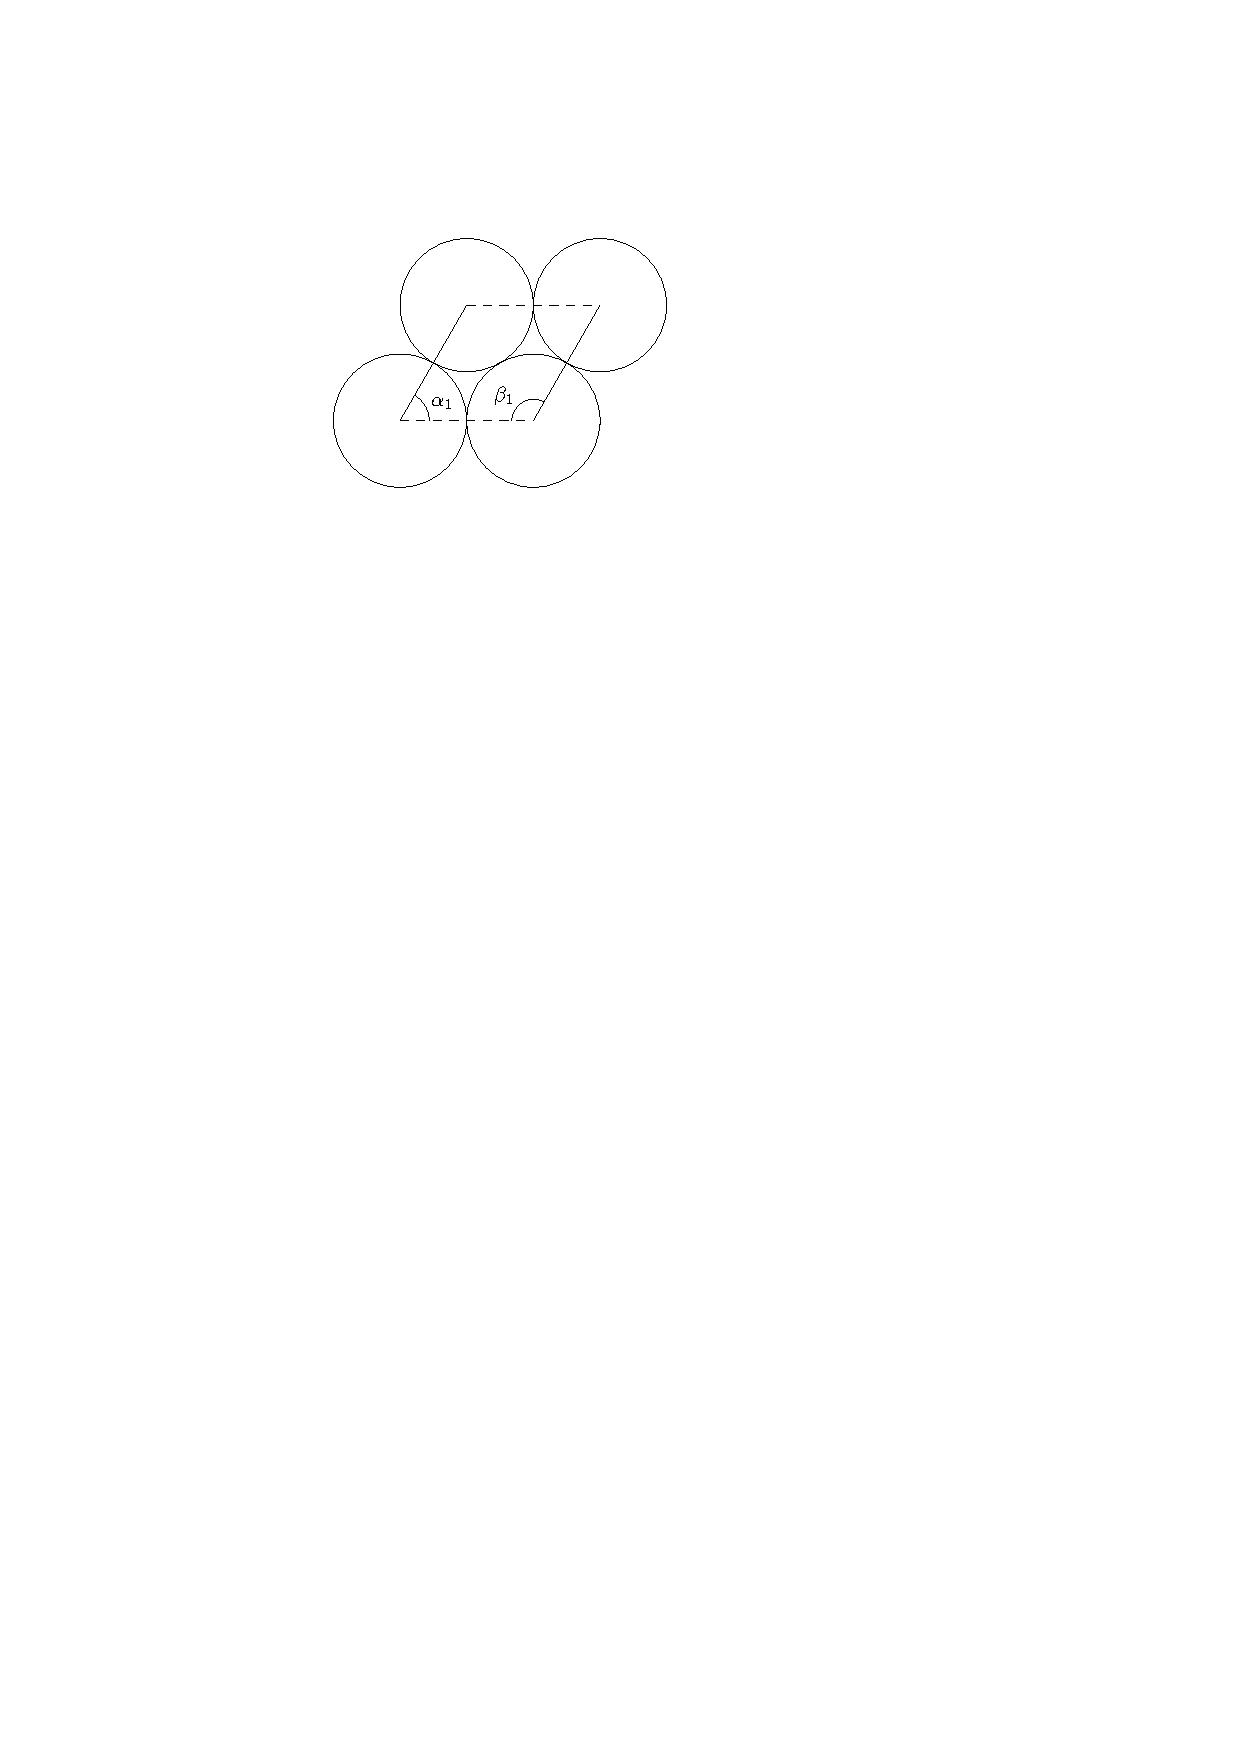
\includegraphics[width=.33\columnwidth]{graphics/PerturbedVertebrae.pdf}
\captionof{figure}{}\label{fig:PerturbedVertebrae.pdf}
\end{center}
\end{minipage}

In this case we will show that the distances between the centers of neighboring disks are small relatively to canonical position of a perfect snowflake, i.e.
\begin{lem}\label{lem:disksOfPathways}
For any realized perturbed snowflake $S_i$, the distance between disks $D_{k,j}$, $D_{k+1,j}$, $D_{k+1,j+1}$, and $D_{k,j+1}$ are relatively small with respect to the relative distance in a perfect snowflake where $k = 1$, $\dots$, $6$ and $j = 2$, $\dots$, $i$.
\end{lem}
\end{enumerate} 

We will show the proofs of Lemmas \ref{lem:s1Small} through \ref{lem:disksOfPathways} later on.


\begin{minipage}{\linewidth}
\begin{center}
\includegraphics[width=.66\columnwidth]{graphics/ch4Paralellogram.pdf}
\captionof{figure}{}\label{fig:ch4Paralellogram.pdf}
\end{center}
\end{minipage}
% In Figure \ref{fig:modifiedContactGraph.pdf}, we have a realization of disk arrangement from a perturbed snowflake.
% In a disk arrangement of a perfect snowflake, the disks around the central disk contact the adjacent disks.
% The disk arrangement from the perturbed snowflake does not have this quality.  
% Figure \ref{fig:modifiedContactGraph.pdf} shows a gap $\epsilon(\gamma)$ between adjacent disks around the central disk.  
% This gap is formed from the perturbed weight $\frac{1}{2} + \gamma$ of the central disk.  
% \begin{equation}\label{eqn:epsilonGamma}
% \epsilon(\gamma)=2\gamma + \gamma^2
% \end{equation}
% As the perturbed snowflake grows outer layers, we can begin to define parts of the snowflake and the corresponding disk arrangement.  
% Let the arms extending from the center of a snowflake be \textit{dendrites} and the arms extending off of arms be \textit{metadendrites}.
% In a perturbed snowflake, the dendrites and metadendrites have some freedom to about the plane.  our
% \begin{minipage}{\linewidth}
% \begin{center}
% \includegraphics[width=.66\columnwidth]{graphics/PerturbedContactGraphAnatomy.pdf}
% \captionof{figure}{}\label{fig:PerturbedContactGraphAnatomy.pdf}
% \end{center}
% \end{minipage}
% In Figure \ref{fig:PerturbedContactGraphAnatomy.pdf}, we show an overlay of a realization of a perturbed snowflake, a corresponding disk arrangement, and concentric hexagons about the $v_0$.




% \begin{lem}\label{lem:cg-1}
% Given any realization of a perturbed snowflake of 7 weighted vertices, with the central vertex $v_0$ weighted $\frac{1}{2} + \gamma$ and the others weighted $\frac{1}{2}$, the total additional distance between all vertices is $6 \epsilon(\gamma)$ compared to a perfect snowflake of 7 unit weight vertices.
% \end{lem}
% \begin{proof}
% Consider a canonical disk arrangement of a perturbed snowflake of 7 weighted vertices (see Figure \ref{fig:modifiedContactGraph.pdf}).
% The side length of the sides formed between the center of the central disk and two adjacent disks around the central disk is $1 + \gamma$.  
% Let the distance between the two adjacent disks be $1 + \epsilon(\gamma)$.
% There are a total of $6 \epsilon(\gamma)$ between adjacent centers of disks. 
% The total perimeter of the hexagon formed about the centers of the disks in contact with the central disk is $6 + 6\epsilon(\gamma)$. 
% Note that 1) the total perimeter of the hexagon formed on a perfect snowflake of 7 weighted vertices is 6 and 2) the canonical disk arrangement can be transformed to any other disk arrangement corresponding to the perturbed snowflake of 7 weighted vertices by pushing the the ring of disks around the central disk together such that all adjacent disks are in contact with each other with the exception of the disks at the end.
% \end{proof}

%  \section{On the Decidability of Problem \ref{problem:UnorderedContactGraph}}
% \begin{proof} 
% Consider a $k \times (\sqrt{3}k)$ rectangle section of a triangular lattice, and place disks of radius 1 at each grid point as in Fig. ?????. 
% The contact graph of these disks contains 2-cycles. 
% Consider the spanning tree $T$ of the contact graph indicated in Fig. ????. 
% The tree $T$ decomposes into paths of collinear edges: $T$ contains two paths along the two main diagonals, each containing $2k - 1$ vertices; all other paths have an endpoint on a main diagonal. 
%  We now modify the disk arrangement to ensure that its contact graph is $T$. 
%  The disks along the main diagonal do not change. 
%  We reduce the radii of all other disks by a factor of $1 - k^{-3}$ (as a result, they lose contact with other disks), and then successively translate them parallel in the direction of the shortest path in $T$ to the main diagonal until the contact with the adjacent disk is reestablished. 
%  The Hausdorff distance between the union of these disks and the initial $k \times (\sqrt{3}k)$ rectangle is clearly less than 1.
%  However, the contact tree $T$ with these radii no longer has a unique realization (small perturbations are possible). 
%  To show stability, we argue by induction on the hop distance from the central disk. 
%  There are $O(i)$ disks at i hops from the central disk, most one which have radius $(1-k^{-3}) \frac{1}{2}$.
%  Since all radii are 1 or $(1-k^{-3}) \frac{1}{2}$,the six neighbors of the central disk can differ from the regular hexagon by at most $O(k )$. 
%  Similarly, the disks at $i$ hops from the center be off from the triangular grid pattern by $O(i2^{k-3})$, for $i = 1,2,\dots,k$.

%  \begin{minipage}{\linewidth}
% \begin{center}
% \includegraphics[width=.66\columnwidth]{graphics/ch4Paralellogram.pdf}
% \captionof{figure}{}\label{fig:ch4Paralellogram.pdf}
% \end{center}
% \end{minipage}
% \end{proof}


% Recall that problem (\ref{problem:UnorderedTree}) states: given a positive weighted tree, $T$, is $T$ the contact graph of some disk arrangement where the radii are equal to the vertex weights?  

% \begin{proof}
% Suppose we are given a positive weighted tree, $T = \lr{V_1,E_1}$.  By the Disk Packing Theorem, there is a disk arrangement in the plane, $D$, whose contact graph, $G=\lr{V_2,E_2}$ is isomorphic to $T$.  We need to so that $G=T$ and the radii of the disks in $D$ are equal to the vertex weights of $T$.

% To show that $G=T$, we need to show that $V_1=V_2$ and $E_1=E_2$.  

% To show that the radii of the disks in $D$ are equal to the vertex weights of $T$, we first consider ....  
% \end{proof}

% Related Previous Work. Polygonal linkages (or body-and-joint frameworks) are a gen-
% eralization of classical linkages (bar-and-joint frameworks) in rigidity theory. A linkage
% is a graph G = (V, E) with given edge lengths. A realization of a linkage is a (crossing-
% free) straight-line embedding of G in the plane. Bhatt and Cosmadakis [3] proved that
% the realizability of linkages is NP-hard. Their “logic engine” method [11, 13, 15, 18],
% has become a powerful tool in graph drawing. The logic engine is a graph composed
% of rigid 2-connected components, connected by cut vertices (hinges). The two possi-
% ble realizations of each 2-connected component (that differ by a single reflection) rep-
% resent the truth assignment of a binary variable. This method does not applicable to
% the oriented version of the realizability, where the circular order of the neighbors of
% each vertex is part of the input. Cabello et al. [6, 14] proved that the realizability of 3-
% connected linkages (where the orientation is unique by Steinitz’s theorem) is NP-hard,
% but efficiently decidable for near-triangulations [6, 12].
% Note that every tree linkage can be realized in R2 (with almost collinear edges).
% According to the celebrated Carpenter’s Rule Theorem [9, 21], every realization of a
% path (or a cycle) linkage can be continuously moved (without self-intersection) to any
% other realization. In other words, the realization space of such a linkage is always con-
% nected. However, there are trees of maximum degree 3 with at few as 8 edges whose
% realization space is disconnected [2]; and deciding whether the realization space of a
% tree linkage is connected is PSPACE-complete [1]. (Earlier, Reif [20] showed that it is
% PSPACE-complete to decide whether a polygonal linkage can be moved from one re-
% alization to another among polygonal obstacles in R3.) Cheong et al. [7] considers the
% “inverse” problems of introducing the minimum number of point obstacles to reduce
% the configuration space of a polygonal linkage to a unique realization.
% Connelly et al. [10] showed that the Carpenter’s Rule Theorem generalizes to certain
% polygonal linkages, which are obtained by replacing the edges of a path linkage with
% special polygons called (slender adornments). Our Theorem 1 indicates that if we are
% allowed to replace the edges of a path linkage with arbitrary convex polygons, then
% deciding whether the realization space is empty or not is already NP-hard.
% Recognition problems for intersection graphs of various geometric object have a
% rich history [18]. Breu and Kirkpatrick [5] proved that it is NP-hard to decide whether
% a graph G is the contact graph of unit disks in the plane (a.k.a. recognizing coin graphs
% is NP-hard). A simpler proof was later provided via the logic engine [13]. It is also NP-
% hard to recognize the contact graphs of pseudo-disks [18] and disks of bounded radii [4]
% in the plane, and unit disks in higher dimensions [17, 18]. All these hardness reductions
% produce graphs of high genus, and do not apply to trees. Note that the contact graphs
%  of disks (of arbitrary radii) are exactly the planar graph (by Koebe’s circle packing
%  theorem), and planarity testing is polynomial. Consequently, every tree is the contact
%  graph of disks of some radii in the plane.


%My goals for next week are as follows:
%1) Clean up chapter 1.  This will happen over the next several weeks.
%2) Continue section 2.3
%3) Add graphics to epsilon-approximation definition to facilitate the explanation.
%4) Anything else  I have time for.



% $\overline{v_0 }$

%Define the snowflake graph, S_i, without pictures
%v_0 has six paths attached to it, p_1, p_2, ..., p_6.  Each path has i vertices.
%for every other path p_1, p_3, and p_5 ,
%	Each vertex on that path has two paths attached, one path on each side of p_k.
%	The number of vertices that lie on the path attached to the j^{th} vertex of p_k is $i-j$
%Let all vertices on the contact graph have weight 1 except $v_0$ whose weight is 1 + \epsilon.
%For any $i$, the weighted contact graph $S_i$, is a subgraph of the unit distance graph of the triangular lattice
%lattice be V = {a(1,0) + b(1/2, \frac{\sqrt{2}}{3} such that a,b \in \bbZ}
%		  E = {{u,v} such that u,v \in V and ||u-v||=1}
%Define this as a canonical position of the disks corresponding to the vertices; goal: show every realization of S_i's disks is close to the canonical position of the disk under hausdorff distance (see lemma)
%NTS: there exists a disk arrangement that corresponds to this weighted contact graph, S_i
%pf:For any two adjacent stems are disjoint, angular displacement and planar (point) displacement
  

%    \begin{prob}[Unordered Realizibility Problem for the Tree]\label{problem:UnorderedTree}
%    For a tree with positive weights for the verticies, it asks whether it is a contact graph of some 
%    disk arrangement where the radii are equal to the vertex weights.
%    \end{prob}
%    
%    \begin{prob}[Ordered Realizibility Problem for the Tree]\label{problem:OrderedTree}
%    For a tree with positive weights for the vertices, it asks whether its corresponding graph is the 
%    ordered contact graph of some disk arrangement where the radii equal the vertex weights.
%    \end{prob}

\section{Proofs of Lemmas \ref{lem:s1Small} through \ref{lem:disksOfPathways}}
We now prove the Lemmas \ref{lem:s1Small} through \ref{lem:disksOfPathways}.
\subsection{Proof of Lemma \ref{lem:s1Small}}
\begin{proof}
Recall that we are to show that for any realized perturbed snowflake $S_i$, the gaps created in subset $S_1 \subset S_i$ are small.  

\begin{minipage}{\linewidth}
\begin{center}
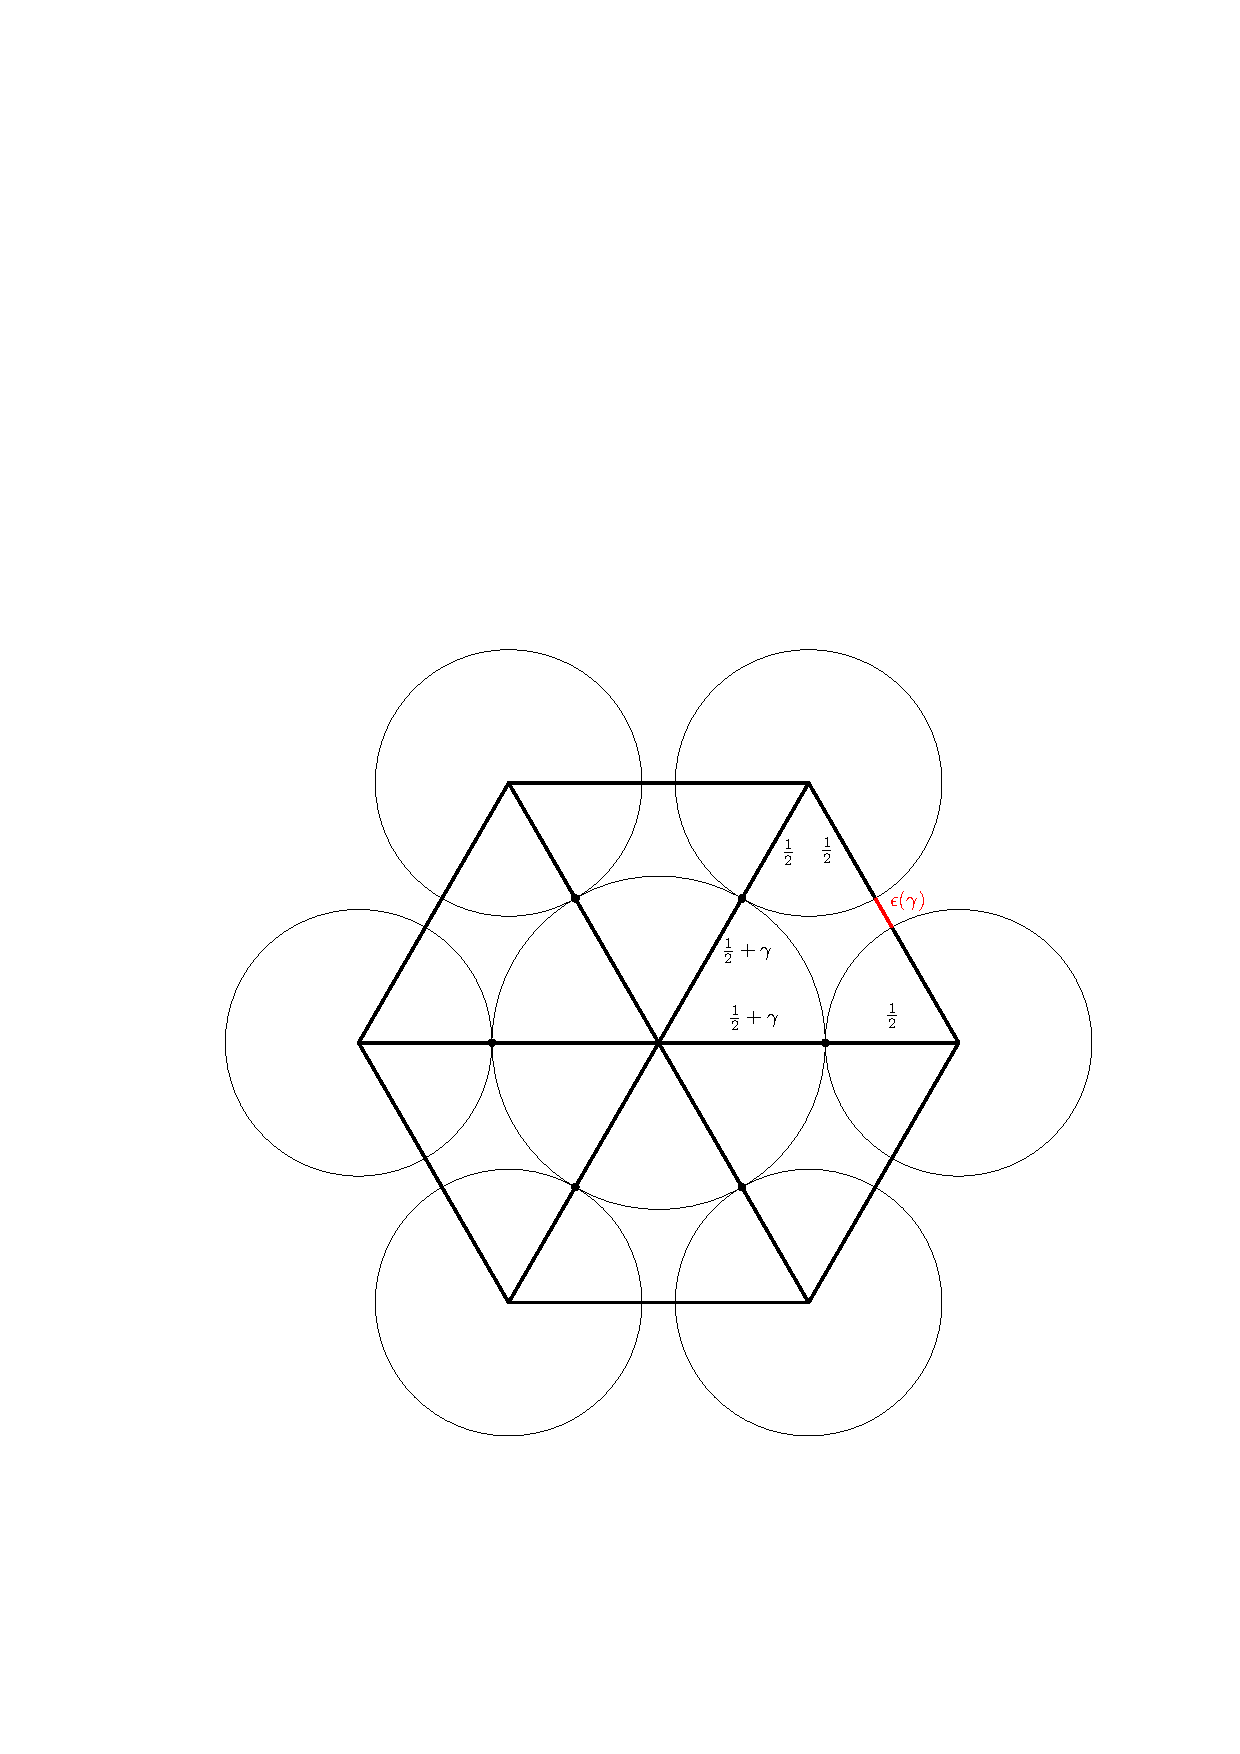
\includegraphics[width=.33\columnwidth]{graphics/modifiedContactGraph.pdf}
\captionof{figure}{A canonical disk arrangement from a perturbed snowflake with 6 unit disks around a central disk with radius $\frac{1}{2} + \gamma$.}\label{fig:modifiedContactGraph.pdf}
\end{center}
\end{minipage}

One way to do this is to demonstration that the sum of gaps for any realization of a contact graph of a perturbed snowflake $S_1$ is small. 
Denote the vertices around $v_0$ as $v_1$ through $v_6$ in a clockwise pattern about $v_0$. 
Without loss of generality, given a realization denote $\epsilon_{k, k+1} (\gamma)\geq 0$ as the gap created between adjacent disks corresponding to $v_1$ thourgh $v_6$.

Consider the realization where $\epsilon_{k, k+1} (\gamma) = 0$ with the exception of $\epsilon_{1,6} >0$.  
That is, ever consecutive pair of disks about the central disk is in contact with each other with the exception of $D_1$ and $D_6$.  
The realization provides 5 congruent triangles between the centers of $D_0$ and $\lr{D_1,D_2}$, $\lr{D_2,D_3}$, $\lr{D_3,D_4}$, $\lr{D_4,D_5}$, and $\lr{D_5,D_6}$.  
Given perturbation $\gamma > 0$, the side lengths between $\lr{D_0,D_i}$ are $1 +\gamma$ and the side length of $\lr{D_i, D_{i+1}}$ is 1.
Using law of cosine the angle formed between $\lr{D_0,D_i}$ and $\lr{D_0,D_{i+1}}$ is $$2 \tan^{-1} \frac{1}{2\lr{1+\gamma}}.$$  
The angle between $\lr{D_6, D_1}$ is $$y=2 \pi - 5 \cdot \lr{2 \tan^{-1} \frac{1}{2\lr{1+\gamma}}}.$$  
The side length of $\lr{D_6, D_1}$ is
$$\sqrt{-2 \, {\left(\gamma + 1\right)}^{2} \cos\left(-10 \,
\arctan\left(\frac{1}{2 \, {\left(\gamma + 1\right)}}\right)\right) + 2
\, {\left(\gamma + 1\right)}^{2}}.$$
Note that as $\gamma \rightarrow 0$, the side length of $\lr{D_6, D_1}$ is approximately 1 + .466861, where $\epsilon(\gamma) \approx .466861$ as $\gamma \rightarrow 0$.
This establishes an upperbound on the maximal displacement about $S_1$ with respect to the side lengths between the centers of disks about $D_0$.

The lower bound is established using the configuration found in Figure \ref{fig:modifiedContactGraph.pdf}.  
he realization provides 6 congruent triangles between the centers of $D_0$ and each disk about $D_0$.
Without loss of generality, to find the side length of between neighboring disks about $D_0$, we find need to $\epsilon(\gamma)$.  
The angle between $\lr{D_0, D_i}$ and $\lr{D_0,D_{i+1}}$ is $\frac{\pi}{3}$; using the law of cosine, we can determine the side length of $\lr{D_i,D_{i+1}}$ is $$\sqrt{1 + 2 \gamma + \gamma^2}.$$  


Thus the perturbation about $S_1$ in and confiugration is bounded and small.
\end{proof}
\subsection{Proof of Lemma \ref{lem:angularArrangement}}
\begin{proof}
Recall that we are to show that for any realized perturbed snowflake $S_i$, the angular value of $\alpha_k$ and $\beta_k$ are small.  
In canoncical position, the angle between $p_{k,j}^+$ and $p_{k,j}^-$ is $\frac{\pi}{3}$.  
In a non-canonical position, we define the change in angle to be $f(\epsilon)$.  
About a 
We prove this with induction. 


\begin{minipage}{\linewidth}
\begin{center}
\includegraphics[width=.66\columnwidth]{graphics/Vertebrae.pdf}
\captionof{figure}{}\label{fig:Vertebrae.pdf}
\end{center}
\end{minipage}

% First consider the changes the angles $\alpha_1$, $\beta_1$, $\alpha_2$, and $\beta_2$.  
$$
\begin{array}{rcl}
\alpha_i +\beta_i &\leq& 120 + f(\epsilon)\\
2 \pi &\leq& \gamma_i + \delta_i + \frac{2 \pi}{3} + f(\epsilon)\\
2 \pi - \lr{\gamma_i + \delta_i} &\leq& \frac{2 \pi}{3} + f(\epsilon)\\
\alpha_{i+1} + \beta_{i+1} &\leq& \frac{2 \pi}{3} + f(\epsilon)\\
\end{array}
$$
\end{proof}
\subsection{Proof of Lemma \ref{lem:disksOfPathways}}
\begin{proof}
Recall that we are to show that for any realized perturbed snowflake $S_i$, the distance between disks $D_{k,j}$, $D_{k+1,j}$, $D_{k+1,j+1}$, and $D_{k,j+1}$ are relatively small with respect to the relative distance in a perfect snowflake where $k = 1$, $\dots$, $6$ and $j = 2$, $\dots$, $i$.

\begin{minipage}{\linewidth}
\begin{center}
\includegraphics[width=.66\columnwidth]{graphics/ch4Paralellogram.pdf}
\captionof{figure}{}\label{fig:ch4Paralellogram.pdf}
\end{center}
\end{minipage}


\end{proof}
% ----------------------------
% CHAPTER 3. (Labels refer to the file cat.pdf)

% Glossary of formulas:
% For arctan, sin, cos, and sec, I would give upper and lower bounds
% (rather than approximate values).
% For example, the Maclaurin series of tan^{-1} gives: x-\frac{x}{3} <
% \tan^{-1}x < x for all 0<x<1.
% All lowerupper bounds are derived from the first or the first two terms
% of the Maclaurin series.


% In (3.5), I would simply (5s^\kappa-1)^3  to (4s^\kamma)^3=4s^{3\kappa},
% which is true for sufficiently large values of s (above a constant
% threshold).
% This will simplify the formulae (3.5)--(3.10).

% Below Figure 3.18, the paragraph title "Vertical Displacement delta" is
% missing.

% Below Figure 3.20. You introduce omega, but you later use omega_i.
% I would define omega_i from the start.

% Below Figure 3.21, you consider the case that omega_i \leq \pi/2.
% It is unclear why the threshold is \pi/2. Shouldn't it be
% \pi/2-2arctan(1/100N), that is \pi/2 minus twice the angle of
% angle of the right triangle shown in the bottom of Figure 3.21?

% Lemma 7, and the calculation above it: I don't understand this lemma.
% I think the main argument should something line this:
% --If omega_i is close to pi, then O_{i+1} has a horizontal displacement
% of about 2 units, and it
% overlaps with another obstacle (which has small displacement by induction).
% --If omega_i is between 0 and pi (but not close to either 0 or pi), then
%   the top vertex of the small rombus is "too high,", contradicting the
% fact the
%    O_{i+1} has "small" vertical displacement (here the terms "too high" and
%    "small" can be quantified in terms of the parameter s).

% -------------------------------------
% CHAPTER 4. OUTLINE

% In chapter 4, we show that for every epsilon>0 there exists an ordered
% weighted tree T_epsilon such that every realization of T_epsilon as an
% ordered disk contact graph, where the radii of the disks equal the
% vertex weights, has Housdorff distance at most epsilon 1 from a regular
% hexagon of unit side length. Once we establish this, we can prove
% Theorem 4 by extending the construction in Section 3 and simulating
% regular hexagons with ordered trees T_epsilon.

% Section 4.1 should define Hausdorff distance and eps-approximation; and
% provide a few examples.

% Section 4.2 should define the snowflake trees. It is an infinite family
% of ordered trees, say T_k,
% where teach axis contains k vertices.

% Section 4.3 should show that for every k, the snowflake tree (with
% vertex weights 1/2+delta and 1/2
% can be realized as a contact graph of disks; and this realization has
% Hausdorff distance at most 1
% from a regular Hexagon (of side length k). Let us also define a
% "canonical position" of the disk
% centers; where each center is a vertex of the hexagonal lattice. Note,
% however, that the canonical
% position does not give a valid realization!

% Section 4.4 should prove that in  _every_ realization of the snowflake
% tree T_k, every disks is "close"
% to their canonical position (here the term "close" must be
% quantified---an upper bound on the maximal distance of a disk from its
% canonical position comes from the proof).

% Section 4.5: Proof of Theorem 4 (this should be rather short: we simply
% state that the construciton of Section 3 can be repeated).

% -----------------------------------
% Lemma 1 in Chapter 4.

% The statement of the lemma is fine, just need to quantify it in terms of
% gamma.

% In the proof of the lemma, the formula
% y = 2\pi - 5( 2 \tan^{-1} frac{1}{2(1+gamma)}
%    = 2\pi - 10 \tan^{-1} frac{1}{2(1+gamma)}
% is great. Observe that if gamma=0, then y=pi/3.
% By continuity, for small values of gamma,
% y will be close to pi/3.

% Note that 1-1/(1+gamma) < gamma.
% Since the derivative of tan^{-1}(x) is less than 1;
% we conclude that  tan^{-1} frac{1}{2(1+gamma)}
% < tan^{-1}(frac{1}{2})  + frac{1}{2}(1-frac{1}{1+ gamma}
% < pi/3 + gamma/2.
% -----------------------------------

% Caterpillar concept:

% A caterpillar can simulate a small rhombus.

% But the main point is Lemma 2 in that paper, which can be used directly
% for the proof of Lemma 2 in Chapter 4 (to show the displacement is small
% for every axis of the snowflake graph. .

% -------------------------------------